% arXiv preprint — Hybrid Post-Quantum Key Exchange for WireGuard
% Compile: tectonic main.tex
\documentclass[11pt,a4paper]{article}

% Math packages first to avoid \Bbbk conflicts with later packages
\usepackage{amsmath,amssymb,amsthm}

% Page geometry — arXiv preprint look
\usepackage[margin=1in,a4paper]{geometry}

% Encoding and fonts
\usepackage[T1]{fontenc}
\usepackage[utf8]{inputenc}
\usepackage{lmodern}
\usepackage{microtype}

% Allow a little extra stretch to absorb tightly-packed \texttt{} and inline math
\emergencystretch=3em
\tolerance=1500

% Tables and figures
\usepackage{booktabs}
\usepackage{graphicx}
\usepackage{float}
\usepackage{multirow}
\usepackage{array}

% Lists
\usepackage{enumitem}

% URLs and references — xcolor needed for hyperref's mix syntax
\usepackage[dvipsnames]{xcolor}
\definecolor{linkblue}{rgb}{0.15,0.30,0.60}
\usepackage[colorlinks=true,
            linkcolor=linkblue,
            citecolor=linkblue,
            urlcolor=linkblue,
            pdftitle={Hybrid Post-Quantum Key Exchange for WireGuard: Integrating ML-KEM into a Production Rust Userspace Implementation},
            pdfauthor={Mihai-Cristian Farcaș}]{hyperref}
\usepackage[capitalize,noabbrev]{cleveref}

% Bibliography style
\usepackage[numbers,sort&compress]{natbib}

% Pretty section heads — preprint style
\usepackage{titlesec}
\titleformat{\section}
  {\normalfont\Large\bfseries}{\thesection}{1em}{}
\titleformat{\subsection}
  {\normalfont\large\bfseries}{\thesubsection}{1em}{}

% Header/footer — arXiv preprint convention
\usepackage{fancyhdr}
\pagestyle{fancy}
\fancyhf{}
\fancyhead[L]{\small Hybrid Post-Quantum Key Exchange for WireGuard}
\fancyhead[R]{\small Preprint}
\fancyfoot[C]{\thepage}
\renewcommand{\headrulewidth}{0.4pt}
\setlength{\headheight}{14pt}

% Re-use thesis figures
\graphicspath{{../../thesis/figures/}}

\title{\textbf{Hybrid Post-Quantum Key Exchange for WireGuard:\\
Integrating ML-KEM into a Production Rust Userspace Implementation}}

\author{
  Mihai-Cristian Farca\textcommabelow{s}\\
  Babe\textcommabelow{s}-Bolyai University\\
  Cluj-Napoca, Romania\\
  \texttt{mihaicristianfarcas@gmail.com}
}

\date{\today}

\begin{document}
\maketitle

\begin{abstract}
WireGuard is now the dominant modern VPN protocol, valued for its small codebase, strong cryptography, and high performance. Its key exchange, however, relies entirely on X25519, which Shor's algorithm will break once a cryptographically relevant quantum computer exists. Under the harvest-now-decrypt-later threat model, adversaries may already be recording WireGuard-encrypted traffic today for future decryption, making migration urgent rather than speculative. NIST finalized FIPS~203 in August 2024, standardizing ML-KEM (Module Lattice-based Key Encapsulation Mechanism), derived from CRYSTALS-Kyber. This paper integrates ML-KEM-768 alongside X25519 into WireGuard's Noise IK handshake, producing a hybrid post-quantum key exchange. The implementation targets BoringTun, Cloudflare's production Rust userspace WireGuard, and is deployable without kernel modifications. A simpler baseline that injects ML-KEM-derived keying material into WireGuard's existing preshared-key (PSK) slot is also implemented as a lower bound on engineering effort. Both approaches are evaluated on three platforms (Apple M4, Raspberry Pi 5, AMD Ryzen 7 5700X), measuring handshake latency, transport throughput, primitive-level microbenchmarks, MTU behaviour, RTT/loss tolerance, per-peer memory footprint, and denial-of-service asymmetry under a saturating handshake flood. An informal security argument shows the hybrid construction to be secure as long as at least one of X25519 or ML-KEM remains unbroken, and to provide per-session forward secrecy that the PSK-slot approach cannot match. To our knowledge, this is the first FIPS~203-compliant hybrid WireGuard implementation built on a production Rust codebase.

\vspace{0.5em}
\noindent\textbf{Keywords:} Post-Quantum Cryptography, WireGuard, ML-KEM, FIPS 203, Hybrid Key Exchange, Noise Protocol, Rust, BoringTun.
\end{abstract}

\section{Introduction}
\label{sec:introduction}

Public-key cryptography underpins virtually all secure communication on the internet: VPN tunnels, TLS handshakes, SSH connections all depend on the computational hardness of problems like integer factorization and the elliptic-curve discrete logarithm. This assumption has held for decades, but will not hold forever. Shor's polynomial-time quantum algorithm~\cite{shor1994algorithms} solves both problems, so a sufficiently large fault-tolerant quantum computer would break RSA and elliptic-curve cryptography. Current estimates put the cost of factoring RSA-2048 at roughly millions of physical qubits with today's error-correction techniques~\cite{gidney2021factor}, and hardware roadmaps from IBM, Google, and others suggest that scale could be reached within the next decade or two.

In response, NIST launched its Post-Quantum Cryptography (PQC) Standardization Project in 2016 and finalized the first round of standards in August 2024: FIPS 203 (ML-KEM, key encapsulation)~\cite{fips203}, FIPS 204 (ML-DSA, digital signatures), and FIPS 205 (SLH-DSA, hash-based signatures). For VPN key exchange, ML-KEM is the directly relevant standard. NIST has also set a hard timeline: classical key exchange algorithms are to be deprecated by 2030 and disallowed entirely by 2035~\cite{nistir8547}.

WireGuard~\cite{donenfeld2017wireguard} is among the most important migration targets. Since 2017 it has largely replaced IPsec and OpenVPN as the go-to VPN protocol, thanks to its small codebase, strong performance, and easy auditability. It ships in the Linux kernel, runs on every major operating system, and is deployed at scale by Cloudflare, Mullvad, NordVPN, Tailscale, and many enterprises. WireGuard's cryptographic design is deliberately opinionated, however: a fixed cipher suite with no negotiation. This rigidity is a security advantage (cipher agility has been a recurring source of vulnerabilities in TLS and IPsec), but it makes migration harder, since there is no built-in way to swap in a different key exchange algorithm.

WireGuard does provide two natural handles for post-quantum augmentation. The first is the preshared-key (PSK) slot, a 256-bit symmetric key that is mixed into the handshake's key derivation chain. If a post-quantum KEM is used out-of-band to establish this PSK, the resulting handshake is quantum-resistant against passive adversaries, at the cost of requiring separate key distribution infrastructure. The second approach is to modify the Noise IK handshake itself, embedding ML-KEM operations alongside the existing X25519 exchange so that both shared secrets contribute to the final session key in every handshake. The latter is what we call the \emph{full hybrid} approach.

\paragraph{Contributions.}
This paper makes four contributions:
\begin{enumerate}[leftmargin=*,topsep=2pt,itemsep=2pt]
  \item A \textbf{PSK-slot baseline}: a small CLI tool that performs ML-KEM-768 key encapsulation between two peers out-of-band and feeds the resulting 256-bit key into BoringTun's \texttt{preshared\_key} field.
  \item A \textbf{full hybrid handshake}: a modified BoringTun whose handshake module runs both X25519 and ML-KEM-768 in every handshake, mixing both shared secrets into the Noise chaining key via HMAC-BLAKE2s, with no changes to the data-transport phase.
  \item A \textbf{three-platform empirical evaluation} on Apple M4, Raspberry Pi 5, and AMD Ryzen 7 5700X, covering handshake latency, transport throughput, primitive-level microbenchmarks, an ML-KEM parameter-set sweep, a path-MTU sweep, an RTT$\times$loss matrix, per-peer memory footprint, and DoS asymmetry under a saturating handshake flood.
  \item An \textbf{informal security argument} comparing the two approaches, with a discussion of where each one fits in practice and what is required to extend authentication to the post-quantum setting.
\end{enumerate}

The rest of the paper is structured as follows.
\Cref{sec:background} covers the relevant background;
\cref{sec:related} surveys prior work;
\cref{sec:design} describes the hybrid design;
\cref{sec:implementation} the BoringTun integration;
\cref{sec:security} the security argument;
\cref{sec:evaluation} the empirical evaluation;
\cref{sec:discussion} discusses deployability and future work;
and \cref{sec:conclusion} concludes.

\section{Background}
\label{sec:background}

\subsection{The quantum threat and HNDL}

All widely deployed public-key cryptography relies on computational hardness assumptions. RSA depends on integer factorization; Diffie-Hellman and its elliptic-curve variants (including X25519, as used in WireGuard) depend on the discrete logarithm problem. Shor's algorithm~\cite{shor1994algorithms} upends this, with a polynomial-time quantum solution to both problems. Concretely, such a machine could derive an X25519 private key from the corresponding public key and reconstruct any session key derived from it. Gidney and Eker\aa~\cite{gidney2021factor} estimate that RSA-2048 could be factored with roughly 20 million noisy qubits in a matter of hours.

What makes this urgent is the \emph{harvest-now-decrypt-later} (HNDL) attack model. An adversary who lacks a quantum computer today can still passively record encrypted traffic --- WireGuard handshakes, transport data, all of it --- and store it cheaply. Once a sufficiently powerful quantum computer is available, the adversary recovers X25519 private keys from stored public keys, reconstructs the ephemeral shared secrets, and decrypts everything. The uncomfortable implication is that traffic encrypted today with classical-only key exchange may already be compromised in a meaningful sense, even though the quantum computers needed to exploit it do not yet exist.

Symmetric cryptography is largely safe. Grover's algorithm provides only a quadratic speedup for brute-force search, effectively halving key lengths. AES-256, ChaCha20-Poly1305, BLAKE2s, and the HMAC-based key derivation used by WireGuard remain unaffected. The migration problem is confined to the asymmetric key exchange layer.

\subsection{WireGuard and the PSK slot}

WireGuard~\cite{donenfeld2017wireguard} is a layer-3 VPN protocol built around a small set of modern cryptographic primitives and a deliberately minimal state machine. The handshake uses Trevor Perrin's Noise Protocol Framework~\cite{noise-protocol} (specifically the IK pattern) with X25519 for Diffie-Hellman, HKDF~\cite{rfc5869} for key derivation, ChaCha20-Poly1305 for authenticated encryption, and BLAKE2s for hashing. The handshake produces a 1-RTT session: the initiator sends one message that authenticates its identity and commits an ephemeral key; the responder verifies and replies; both sides derive matching session keys. Transport flows in UDP packets with a per-message nonce. Sessions rekey after 120 seconds or after $2^{60}$ messages, whichever comes first, and all ephemeral keys are zeroed after use.

WireGuard includes an optional 256-bit preshared key (PSK), added specifically as a transitional measure for post-quantum protection. When configured, the PSK is mixed into the HKDF chain during the handshake, adding a layer of symmetric-key cryptography on top of the X25519 exchange. The design intent is that even if a quantum computer eventually breaks X25519, an attacker who did not also obtain the PSK at the time of the session cannot decrypt the traffic. The PSK mechanism's limitations are structural: it is a long-lived static value, not an ephemeral secret, so it does not provide forward secrecy for the quantum-resistant component, and its distribution and rotation requires an out-of-band channel.

\subsection{Noise and the KEM/DH asymmetry}

Noise patterns specify the sequence of handshake messages along with the Diffie-Hellman operations performed at each step. WireGuard uses the IK pattern --- \emph{I} for the initiator's static (transmitted immediately, encrypted) and \emph{K} for the responder's static (known to the initiator beforehand). Noise protocols maintain a chaining key $\mathit{ck}$ and handshake hash $h$; each DH operation, public key, and encrypted payload is mixed into these values via HMAC and BLAKE2s, building a transcript hash that binds all handshake messages together.

The main difficulty in migrating Noise to PQC is that the design is tied to the algebraic properties of Diffie-Hellman. DH provides non-interactive key exchange: from the other party's public key and one's own private key, either party can compute the shared secret without further interaction. KEMs work differently: one party generates a ciphertext that encapsulates a secret to a specific public key, and only the holder of the corresponding private key can decapsulate it. This asymmetry means the handshake flow needs to be reworked when KEMs are introduced.

\subsection{ML-KEM (FIPS 203)}

ML-KEM was standardized as FIPS 203 in August 2024~\cite{fips203}. It is a key encapsulation mechanism derived from CRYSTALS-Kyber~\cite{bos2018crystals}, whose security rests on the Module Learning With Errors (MLWE) problem~\cite{langlois2015worst}. A KEM exposes three operations: KeyGen produces an encapsulation key and a decapsulation key; Encaps takes an encapsulation key and returns a ciphertext plus a shared secret; Decaps takes the decapsulation key and the ciphertext and recovers the same shared secret.

FIPS 203 specifies three parameter sets: ML-KEM-512 (NIST security category 1, $\sim$AES-128), ML-KEM-768 (category 3, $\sim$AES-192), and ML-KEM-1024 (category 5, $\sim$AES-256). Encapsulation key and ciphertext sizes are 800/768~B, 1184/1088~B, and 1568/1568~B respectively. All three produce a 32-byte shared secret. NIST recommends ML-KEM-768 as the default. On the implementation side, ML-KEM benefits from the Number-Theoretic Transform (NTT), which gives it a raw speed advantage over elliptic-curve operations on commodity CPUs, though that advantage is partly offset by the much larger key and ciphertext sizes.

\subsection{Hybrid key exchange and concatenate-then-KDF}

Hybrid key exchange combines two or more key agreement algorithms so the resulting key is secure as long as at least one component holds. The motivation is straightforward: ML-KEM, though now standardized, has seen far less cryptanalytic scrutiny than X25519. Running both in parallel means a breakthrough against either one alone does not compromise security. The standard construction is the \emph{concatenate-then-KDF} pattern, formalized in NIST SP 800-56C Rev.~2~\cite{nist-sp800-56c}: the shared secrets from each component are concatenated, $Z' = Z \| T$, and fed into a single key derivation function. Giacon, Heuer, and Poettering~\cite{giacon2018combiners} prove that the resulting KEM is IND-CPA-secure as long as either component is IND-CPA-secure, with the bound remaining tight even when one component is broken. This is the same pattern used by Cloudflare and Google in TLS 1.3 and by the IETF hybrid TLS design draft~\cite{ietf-tls-hybrid-design}.

\section{Related Work}
\label{sec:related}

\paragraph{PQ-WireGuard (H\"ulsing et al., 2021).}
The most directly relevant prior work~\cite{hulsing2021pqwireguard} replaces WireGuard's X25519 handshake entirely with a KEM-based construction, with both static-key authentication (Classic McEliece) and ephemeral key exchange (Saber) instantiated post-quantum. Security is proved in the eCK-PFS-PSK model and verified symbolically in Tamarin. This paper differs in three ways: it uses a hybrid construction rather than a pure post-quantum replacement, targets NIST-standardized ML-KEM rather than pre-standardization Saber, and works within the existing BoringTun production codebase rather than a research prototype.

\paragraph{PQNoise.}
Angel, Dowling, H\"ulsing, Schwabe, and Weber~\cite{pqnoise2022} introduce a generic framework for converting Noise patterns into post-quantum equivalents using KEMs, with new token types \texttt{ekem} and \texttt{skem} replacing the two-letter DH tokens. PQNoise also introduces Static-Ephemeral Entropy Combination (SEEC) for hardening KEM randomness. The hybrid construction described here can be viewed as a variant of the \texttt{pqIK} pattern augmented with classical DH.

\paragraph{Hybrid-WireGuard (Lafourcade et al., 2025).}
Lafourcade, Mahmoud, and Ruhault~\cite{lafourcade2025hybrid} revisit PQ-WireGuard with a thorough formal analysis using Sapic+, ProVerif, DeepSec, and Tamarin, and propose two improvements: PQ-WireGuard$\star$ (which fixes a UKS attack on the original) and Hybrid-WireGuard (which combines the DH secrets from WireGuard with the KEM secrets from PQ-WireGuard$\star$). They emphasize that MTU constraints heavily limit which KEMs can be used in WireGuard, since handshake messages need to fit within the IPv6 minimum of 1,280 bytes. This paper builds on their results but takes a different approach: it targets NIST-standardized ML-KEM within the existing BoringTun production codebase, accepts the larger message sizes (relying on IP fragmentation rather than constraining the parameter set), and provides empirical benchmarks on real hardware.

\paragraph{Rosenpass.}
Rosenpass~\cite{rosenpass,rosenpass-github} takes the PSK-slot idea and turns it into a continuously running Rust daemon, generating post-quantum PSKs using Classic McEliece and Kyber-512 and refreshing them every two minutes. Structurally similar to the PSK baseline in this paper but with continuous operation rather than one-time injection. Rosenpass shares the same forward-secrecy limitation as any PSK-based approach.

\paragraph{ExpressVPN's production PSK delivery.}
Membrey and Beyel~\cite{membrey2025expressvpn} describe a production deployment of the PSK-slot approach, using ML-KEM hybrid TLS 1.3 to deliver WireGuard PSKs through a split-service authentication architecture. The system is live across ExpressVPN's global infrastructure, adding 15--20~ms to connection establishment with no steady-state throughput penalty.

\paragraph{Revised PQ-WireGuard with reinforced KEMs.}
Concurrent work by Hashimoto, Katsumata, Niot, and Wiggers (IEEE S\&P 2026)~\cite{hashimoto2026rkem} introduces \emph{reinforced KEMs} (RKEMs). Their Rebar construction eliminates the need for Classic McEliece static keys on the server, reducing the server's public-key memory requirement by 190--390$\times$ and representing the state of the art in purely post-quantum WireGuard design.

\section{Design}
\label{sec:design}

\subsection{Design goals}

The design is guided, in rough order of priority, by: \textbf{correctness} (the hybrid must produce the same session keys at both endpoints and fail securely if either component fails), \textbf{security} (the construction must be secure as long as at least one of X25519 or ML-KEM-768 remains unbroken, and preserve session-key secrecy, perfect forward secrecy, replay resistance, and DoS resistance), \textbf{compatibility} (the PSK-slot baseline must coexist with unmodified WireGuard; the hybrid requires explicit configuration of both parties), \textbf{deployability} (no kernel modifications required), and \textbf{performance} (overhead acceptable on Raspberry-Pi-class hardware).

\subsection{The PSK-slot baseline}

The PSK-slot approach is the minimal intervention: a standalone binary performs ML-KEM-768 key encapsulation between two peers, derives a 256-bit shared secret, and injects it into BoringTun's \texttt{preshared\_key} field. After that, the WireGuard handshake proceeds exactly as in the vanilla case.

Before any WireGuard session is established, the two peers run the PSK exchange out-of-band. One peer generates an ML-KEM-768 keypair and sends the encapsulation key to the other. That peer runs ML-KEM.Encaps, obtaining a ciphertext $\mathit{ct}$ and a 32-byte shared secret $K$, then sends $\mathit{ct}$ back. The first peer runs ML-KEM.Decaps to recover the same $K$. Both peers configure their WireGuard interface with $\texttt{preshared\_key} = K$. The PSK is then mixed into the WireGuard handshake's HMAC-BLAKE2s key derivation chain, providing a quantum-resistant layer of security for all traffic protected by sessions using that PSK.

The PSK baseline has real limitations: the ML-KEM keypair is static or semi-static, so the ML-KEM component provides no forward secrecy. If the PSK is compromised after the fact, all traffic from sessions that used it is exposed. The PSK also has to be distributed before any sessions can be established. The clear advantage: zero changes to WireGuard itself.

\begin{figure}[!ht]
    \centering
    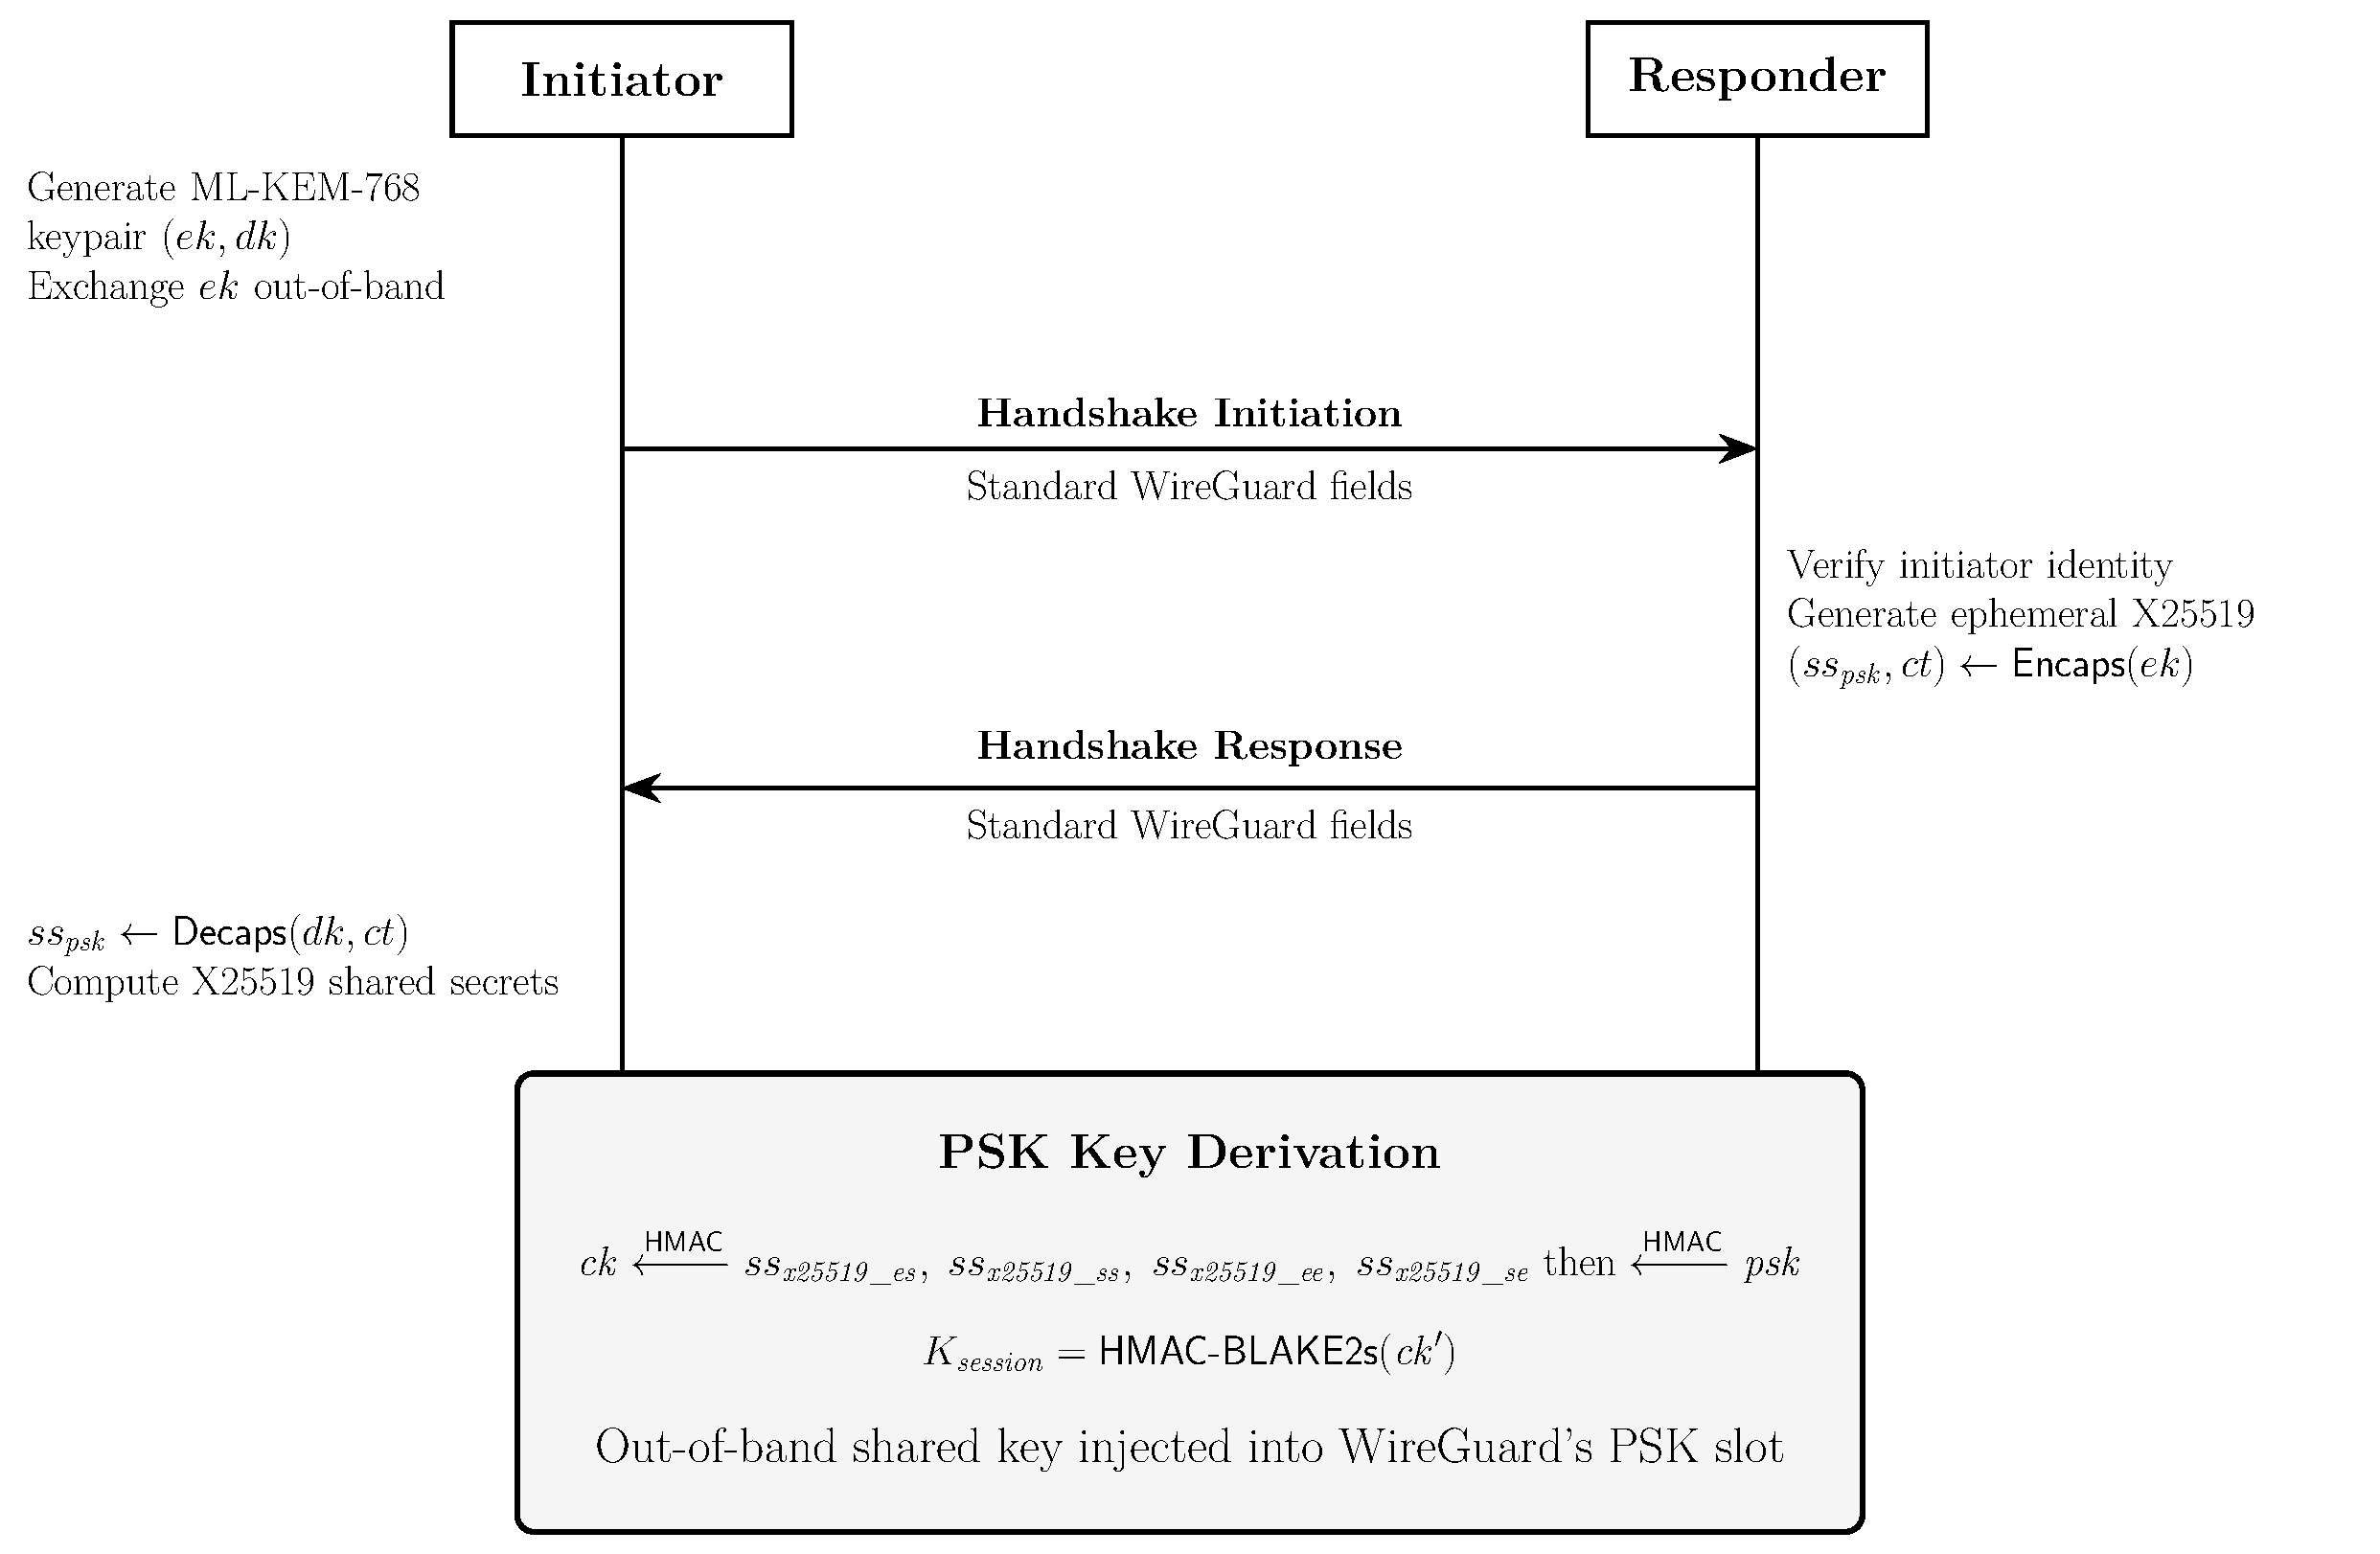
\includegraphics[width=0.85\textwidth]{fig_psk_handshake.pdf}
    \caption{PSK-Slot baseline: out-of-band ML-KEM exchange and PSK injection.}
    \label{fig:psk_handshake}
\end{figure}

\subsection{The hybrid handshake}

The full hybrid integrates ML-KEM-768 directly into the Noise IK handshake. The design follows the concatenate-then-KDF pattern endorsed by NIST SP 800-56C Rev.~2~\cite{nist-sp800-56c} and is structurally similar to the hybrid constructions in TLS 1.3~\cite{ietf-tls-hybrid-design}.

\paragraph{Initiator (first message).}
The initiator generates an ephemeral X25519 keypair as in standard WireGuard. It also generates a fresh ML-KEM-768 keypair for this session: encapsulation key $\mathit{ek}_i$ and decapsulation key $\mathit{dk}_i$. The 1184-byte $\mathit{ek}_i$ is appended to the initiator's first message, after the standard WireGuard fields but before the MAC fields, so that MAC1 and MAC2 cover the entire message, including the ML-KEM material. This ensures the cookie-based DoS-resistance mechanism extends to the post-quantum payload.

\paragraph{Responder (second message).}
The responder processes the X25519 portion of the handshake as in standard WireGuard. It also reads $\mathit{ek}_i$ from the first message, runs $\mathsf{ML\text{-}KEM.Encaps}(\mathit{ek}_i)$ to produce a ciphertext $\mathit{ct}$ (1088 bytes) and shared secret $\mathit{ss}_\mathit{kem}$, and appends $\mathit{ct}$ to the response message.

\paragraph{Initiator decapsulation.}
The initiator reads $\mathit{ct}$ from the response and runs $\mathsf{ML\text{-}KEM.Decaps}(\mathit{dk}_i, \mathit{ct})$, recovering $\mathit{ss}_\mathit{kem}$. Both peers now hold the same $\mathit{ss}_\mathit{kem}$.

\paragraph{Combined key derivation.}
Both parties derive the final session keys by sequentially mixing each shared secret into the Noise chaining key $\mathit{ck}$ via HMAC-BLAKE2s, following the same pattern WireGuard already uses for DH results. The four X25519 shared secrets from the Noise IK pattern ($\mathit{ss}_\mathit{x25519\_es}$, $\mathit{ss}_\mathit{x25519\_ss}$, $\mathit{ss}_\mathit{x25519\_ee}$, $\mathit{ss}_\mathit{x25519\_se}$) are mixed first, exactly as in vanilla WireGuard. Then the ML-KEM shared secret $\mathit{ss}_\mathit{kem}$ is mixed in as an additional step:
\[
\mathit{temp} = \mathsf{HMAC\text{-}BLAKE2s}(\mathit{ck}, \mathit{ss}_\mathit{kem}), \quad
\mathit{ck}' = \mathsf{HMAC\text{-}BLAKE2s}(\mathit{temp}, \mathtt{0x01}).
\]
The handshake hash $h$ is also updated to include the ML-KEM material (both the encapsulation key and ciphertext), binding it to the Noise transcript. The PSK mixing step then proceeds on $\mathit{ck}'$ exactly as in standard WireGuard (using a zero PSK if none is configured). The data-transport phase is unchanged.

This sequential mixing is structurally equivalent to the concatenate-then-KDF pattern from NIST SP 800-56C: each shared secret contributes independently to the chaining key, and the final session keys depend on all components.

\begin{figure}[!ht]
    \centering
    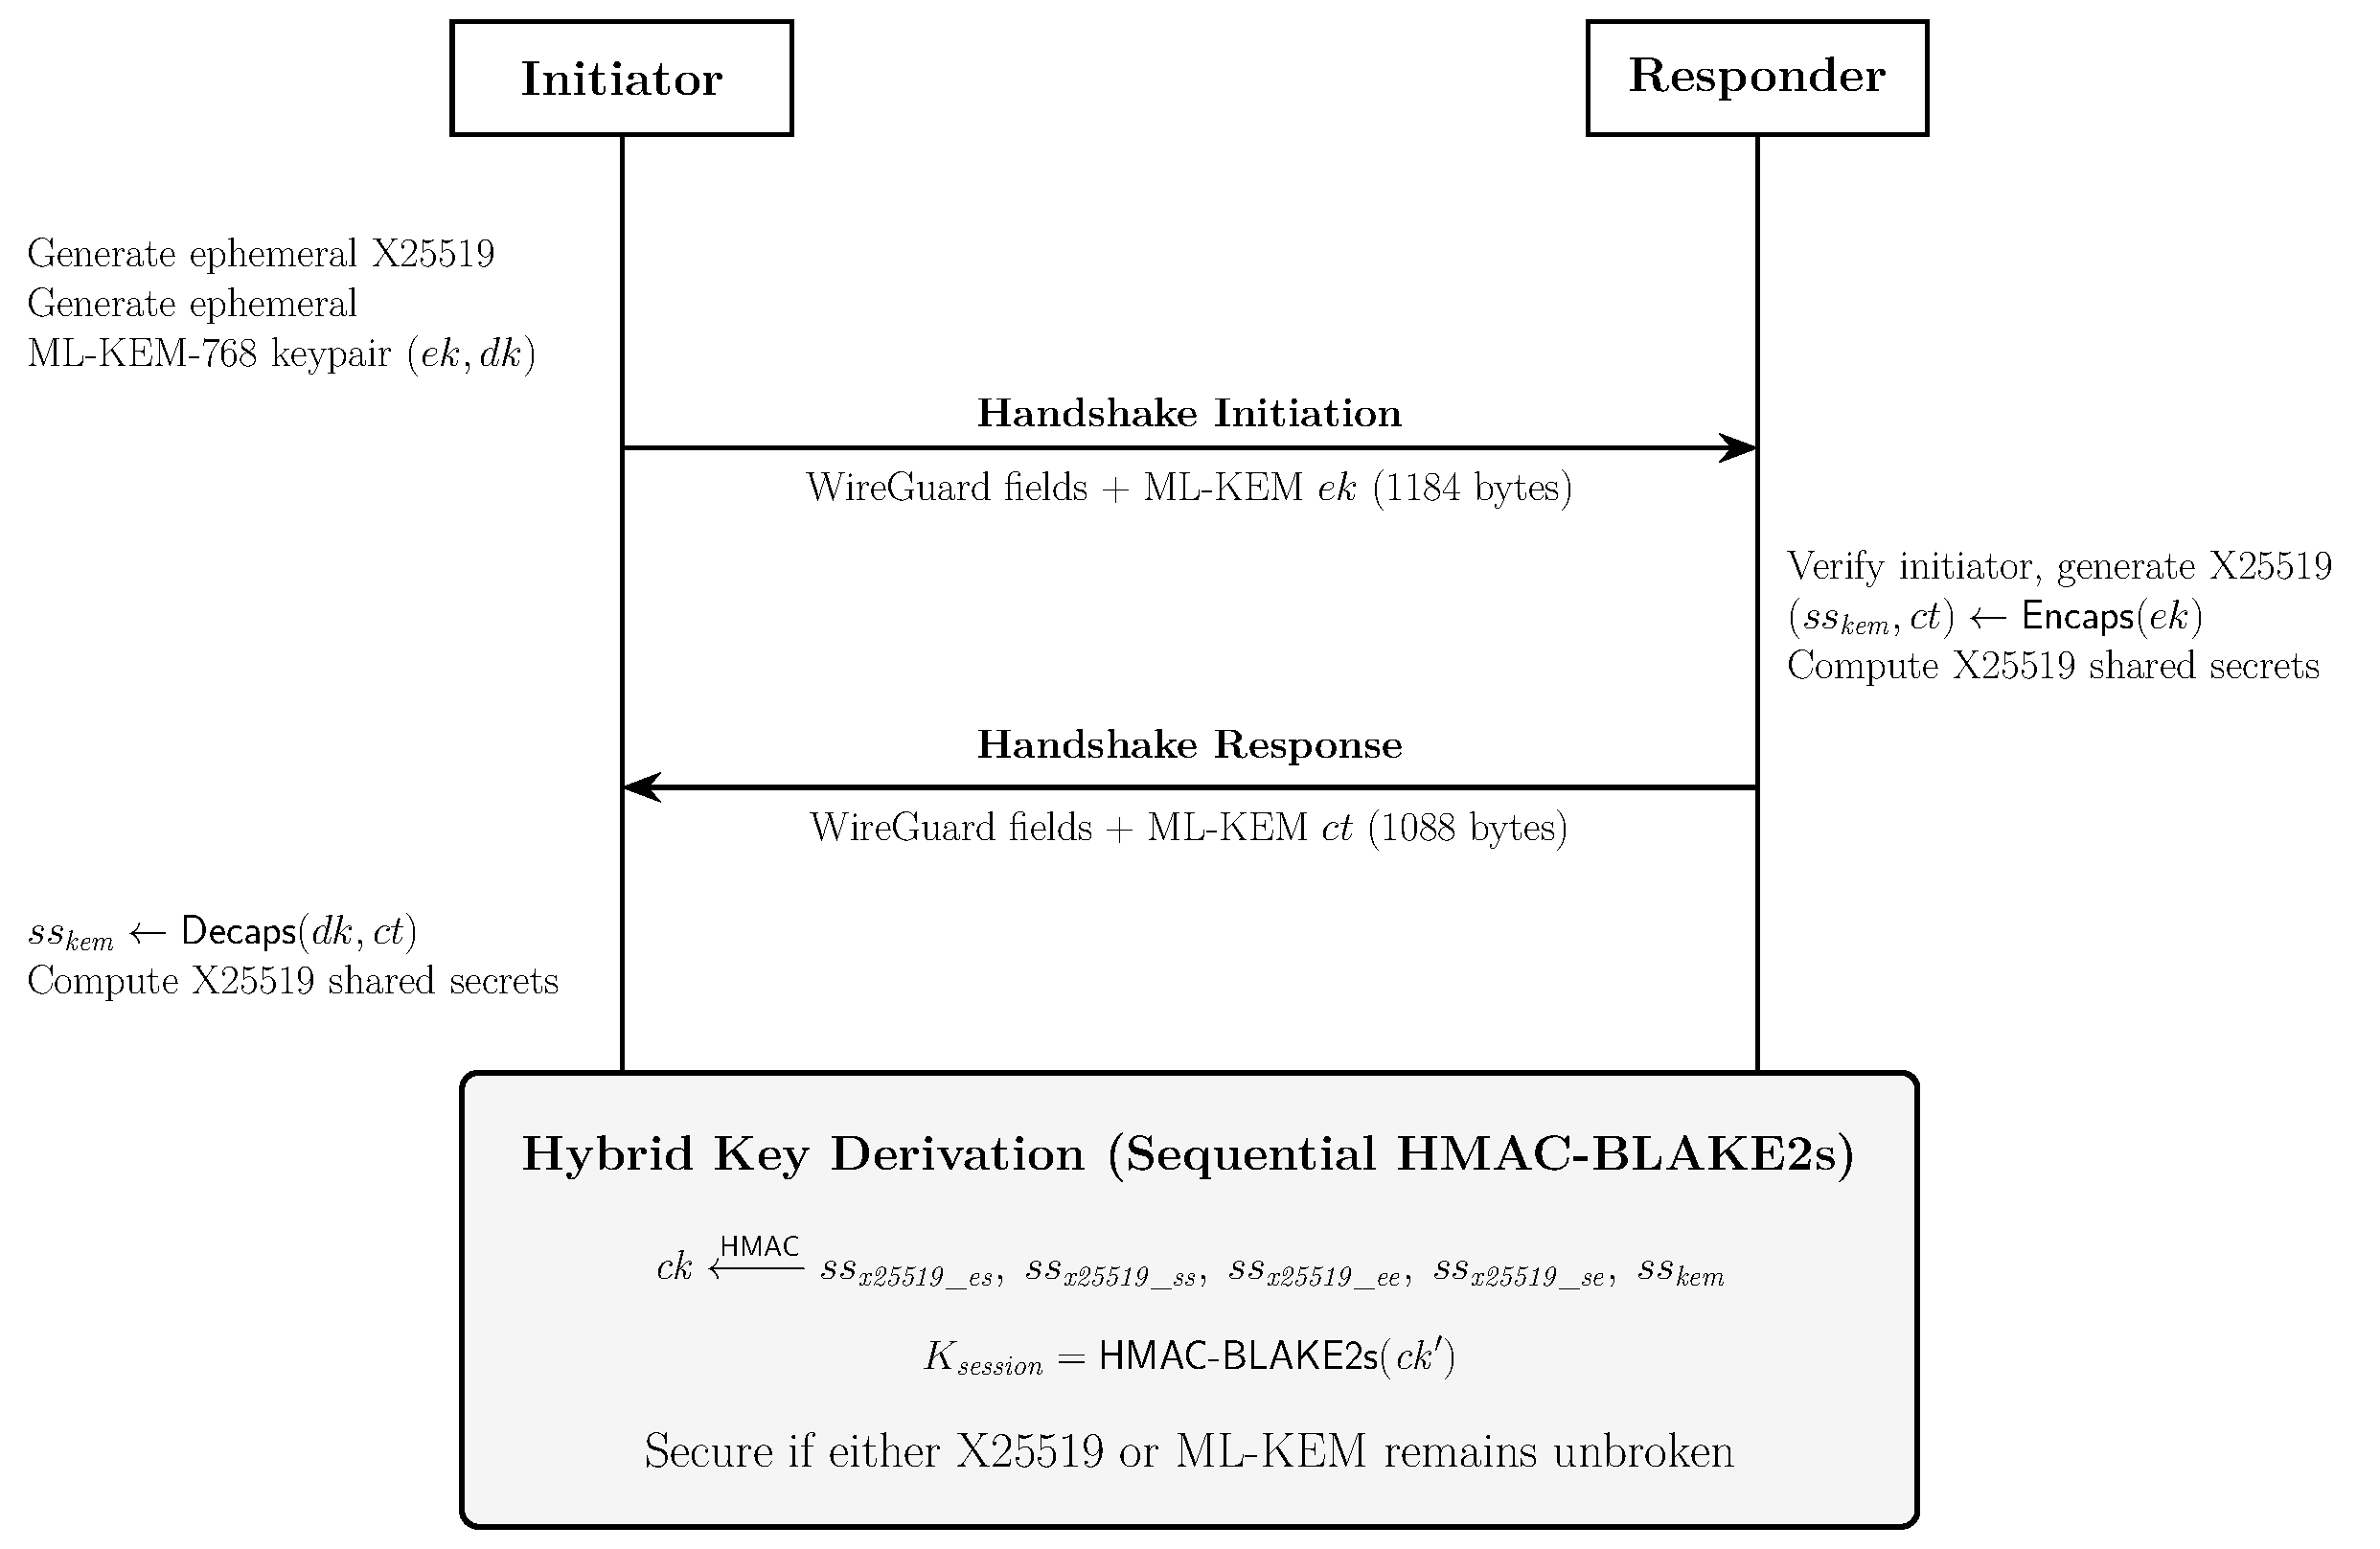
\includegraphics[width=0.85\textwidth]{fig_hybrid_handshake.pdf}
    \caption{The full hybrid handshake: integrated ML-KEM-768 alongside X25519.}
    \label{fig:hybrid_handshake}
\end{figure}

Two properties follow. \textbf{Per-session forward secrecy} comes from both components: the X25519 ephemeral key is fresh for each handshake, and so is the ML-KEM keypair, so $\mathit{ss}_\mathit{kem}$ is unique to each session. The construction is also \textbf{hybrid-secure}: if ML-KEM is completely broken, the session key still depends on the X25519 exchange and cannot be recovered without breaking X25519 too. The converse also holds.

\subsection{Message sizes and MTU}

Vanilla WireGuard's handshake initiation message is 148 bytes and the response is 92 bytes. ML-KEM-768 adds 1184 bytes to the initiation (the encapsulation key) and 1088 bytes to the response (the ciphertext), giving 1332-byte and 1180-byte hybrid messages.

The IPv6 minimum MTU is 1280 bytes, so the hybrid initiation does not fit any IPv6 path without IP-layer fragmentation. UDP does not have application-layer fragmentation, and IP fragmentation is unreliable on real-world paths because some middleboxes drop fragments. The current implementation relies on IP-level fragmentation for oversized handshakes. On typical 1500-byte Ethernet paths, both hybrid messages fit in a single UDP datagram. On constrained paths the initiation fragments at the IP layer; \cref{sec:eval_mtu} reports empirical behaviour. Two alternative strategies (application-level segmentation and Path MTU Discovery with KEM parameter negotiation) are identified as future work in \cref{sec:discussion}.

\section{Implementation}
\label{sec:implementation}

\subsection{BoringTun and the technology stack}

BoringTun~\cite{boringtun} is Cloudflare's userspace WireGuard implementation, written in Rust and deployed on millions of iOS and Android devices and on thousands of Cloudflare Linux servers. It ships as a library crate (\texttt{boringtun}) and a CLI binary (\texttt{boringtun-cli}). The handshake module implements the Noise IK pattern, manages per-peer state machines, performs X25519 operations via the \texttt{x25519-dalek} crate, and uses HMAC-BLAKE2s for chaining key evolution. The transport module (ChaCha20-Poly1305) is not touched.

Rust's ownership and borrowing model rules out buffer overflows, use-after-free, and double-free bugs at compile time, which matters for cryptographic code where such bugs have historically led to exploitable vulnerabilities. It also makes pulling in pure-Rust cryptographic crates from the RustCrypto ecosystem straightforward, with no C FFI boundary.

ML-KEM operations use the \texttt{ml-kem} crate (version 0.3.0-rc.0) from RustCrypto, a pure-Rust, \texttt{no\_std} implementation of FIPS 203 tested against the NIST Known-Answer-Test vectors. Being pure Rust and \texttt{no\_std}, it runs on constrained targets like the Raspberry Pi without any C FFI. Key derivation reuses BoringTun's existing HMAC-BLAKE2s extraction pattern; no separate HKDF or SHA-256 construction is introduced. A small RNG-versioning detail: the \texttt{ml-kem} crate needs \texttt{rand\_core} 0.10, while BoringTun already depends on \texttt{rand\_core} 0.6. Cargo's package renaming feature resolves this: \texttt{rand\_core\_pq} (aliasing 0.10) and \texttt{getrandom\_pq} (aliasing \texttt{getrandom} 0.4) are declared as separate optional dependencies, so both versions coexist in the same binary.

\subsection{Handshake module modifications}

All post-quantum code is conditionally compiled behind a Cargo feature flag (\texttt{pq}). Vanilla builds are completely unaffected: no additional dependencies are compiled, no code paths change, and binary size remains identical. The \texttt{pq} feature gates the \texttt{ml-kem}, \texttt{rand\_core\_pq}, and \texttt{getrandom\_pq} dependencies, as well as all PQ-related message types, state fields, and handshake methods.

\textbf{State extension.} The \texttt{HandshakeState} structure is extended to carry the minimal ML-KEM material each side needs across handshake steps. On the initiator side, only the \texttt{DecapsulationKey768} is stored, so the response can later be decapsulated; the encapsulation key is serialized into the initiation message and then dropped. On the responder side, only the received encapsulation key is stored, so encapsulation can be performed when the response is built; the resulting ciphertext is written directly into the response message rather than retained in state.

\textbf{Message construction.} When the initiator builds the initiation message, it generates a fresh ML-KEM-768 keypair and appends the 1184-byte encapsulation key after the standard WireGuard fields, mixing it into the handshake hash $h$. When the responder processes the initiation, it extracts the encapsulation key, validates its length, runs \texttt{Encaps} to produce $\mathit{ct}$ and $\mathit{ss}_\mathit{kem}$, and appends the 1088-byte $\mathit{ct}$ to the response, again mixing it into $h$.

\textbf{Session-key derivation.} At the end of the handshake, both parties mix $\mathit{ss}_\mathit{kem}$ into the chaining key via the additional HMAC-BLAKE2s step described in \cref{sec:design}, before proceeding to PSK mixing and final session key derivation. A new error variant (\texttt{MlKemDecapsulationFailed}) handles decapsulation failures gracefully, causing the handshake to abort without leaking state.

\textbf{New message types.} Two new message types are introduced: type 5 for PQ handshake initiation (1332 bytes) and type 6 for PQ handshake response (1180 bytes). The packet parser dispatches on message type and size, routing PQ messages to the PQ handshake methods. Vanilla builds reject these message types with \texttt{InvalidPacket}, ensuring graceful interoperability.

\subsection{PSK-slot baseline implementation}

The PSK-slot baseline is implemented as a separate Rust CLI binary, \texttt{pq-psk-tool}, that operates independently of BoringTun. It uses the same \texttt{ml-kem} crate and provides three subcommands implementing a manual three-step ML-KEM-768 key exchange: \texttt{keygen} (generates an ML-KEM-768 keypair, encapsulation key as base64 for transfer, decapsulation seed kept secret), \texttt{encaps <ek\_file>} (runs ML-KEM.Encaps, outputs the ciphertext as base64 and the 32-byte shared secret as a base64 PSK, the format WireGuard's \texttt{wg set} expects), and \texttt{decaps <dk\_file> <ct\_file>} (runs ML-KEM.Decaps, recovers the identical 32-byte PSK). The encapsulation key and ciphertext files are exchanged out-of-band; the tool itself does not implement a network protocol. Both peers then configure their WireGuard interface with the derived PSK using \texttt{wg set <iface> peer <PUBKEY> preshared-key psk.b64}.

\subsection{Test harness}

The \texttt{noise::tests} module contains unit tests for both vanilla and PQ handshake paths, conditionally compiled. They cover PQ handshake message validation (initiation = 1332~B, with the 1180~B response size exercised by the full-handshake test), full PQ handshakes (four-step exchange including keepalive), end-to-end data transport, simultaneous PQ + PSK operation, and verification that a vanilla build rejects PQ message types. A separate shell script automates operational testing on macOS with loopback tunnel, comparison, and demo modes.

\section{Security Analysis}
\label{sec:security}

The security goals for the hybrid handshake are the same as for vanilla WireGuard, as established by Dowling and Paterson's computational proof~\cite{dowling2018wireguard} and Donenfeld and Milner's symbolic Tamarin proof~\cite{donenfeld2018formal}, and extended to the post-quantum setting by PQ-WireGuard~\cite{hulsing2021pqwireguard} and Hybrid-WireGuard~\cite{lafourcade2025hybrid}. We summarize the goals informally and give a hybrid security argument; a fully formal proof in the eCK-PFS-PSK model or in a Sapic+/Tamarin model is left as future work.

\paragraph{Goals.} \textbf{Session-key secrecy}: an adversary who does not corrupt either party's long-term or ephemeral secrets cannot distinguish the established session key from a random value. \textbf{Perfect forward secrecy}: compromise of long-term static keys does not allow decryption of past sessions; each session uses fresh ephemeral keypairs (both X25519 and ML-KEM). \textbf{Post-quantum forward secrecy}: a quantum adversary who breaks X25519 after the session cannot decrypt past traffic, since doing so also requires breaking ML-KEM. \textbf{Authenticity}: both initiator and responder verify each other's identity via X25519 static keys (classical, not post-quantum, in this design). \textbf{DoS resistance}: the WireGuard cookie mechanism is preserved; handshake-init messages with invalid MAC1 are rejected without state allocation. \textbf{Replay resistance}: the handshake transcript, extended to include the ML-KEM material, prevents replay attacks.

\paragraph{Hybrid argument.} Let $\mathit{ss}_\mathit{classical}$ denote the combined X25519 shared secrets and $\mathit{ss}_\mathit{kem}$ the ML-KEM-768 shared secret. After the classical exchange, $\mathit{ck}$ already incorporates $\mathit{ss}_\mathit{classical}$. The ML-KEM secret is then mixed in as
$\mathit{ck}' = \mathsf{HMAC\text{-}BLAKE2s}(\mathsf{HMAC\text{-}BLAKE2s}(\mathit{ck}, \mathit{ss}_\mathit{kem}), \mathtt{0x01})$,
and the session keys $K$ are derived from $\mathit{ck}'$ after the PSK mixing step.

\textbf{Claim:} $K$ is computationally indistinguishable from a random key as long as either $\mathit{ss}_\mathit{classical}$ is pseudorandom (i.e., X25519 is secure) \emph{or} $\mathit{ss}_\mathit{kem}$ is pseudorandom (i.e., ML-KEM-768 is IND-CCA2 secure).

This follows from the security of HMAC-BLAKE2s as a PRF: if either input to the chaining key is uniformly random and independent of the adversary's view, then the chaining-key output and the derived session keys are computationally indistinguishable from random (under the assumption that BLAKE2s is a secure PRF). The sequential mixing of independent shared secrets into the chaining key is structurally equivalent to the concatenate-then-KDF pattern; each component contributes independently to the final key material. The formal proof is a standard hybrid argument; Giacon, Heuer, and Poettering~\cite{giacon2018combiners} give it for the concatenation combiner.

In the HNDL threat model, the adversary captures the handshake transcript, which includes both the X25519 public keys and the ML-KEM ciphertext. With a quantum computer, the adversary can recover $\mathit{ss}_\mathit{classical}$ from the X25519 keys. To also recover $\mathit{ss}_\mathit{kem}$, the adversary must additionally solve the ML-KEM decapsulation problem --- recover $\mathit{dk}_i$ from $\mathit{ek}_i$ and then decapsulate $\mathit{ct}$ --- which is the IND-CCA2 security problem for ML-KEM, believed hard for both classical and quantum adversaries under the MLWE assumption.

\paragraph{Forward secrecy.} In the PSK-slot baseline, the ML-KEM exchange is performed once, out-of-band, and the resulting PSK is reused across many WireGuard sessions. If an adversary compromises the PSK after the fact, all sessions using that PSK are retroactively vulnerable, even to a purely classical adversary. The ML-KEM component does not contribute ephemeral, per-session material. In the full hybrid, $(\mathit{ek}_i, \mathit{dk}_i)$ is generated fresh for every handshake, and $\mathit{ct}$ encapsulates $\mathit{ss}_\mathit{kem}$ specifically for that session's ephemeral key. Once $\mathit{dk}_i$ has been zeroed from memory (consistent with WireGuard's existing practice of zeroing ephemeral keys after use), no information remains that would allow recovery of $\mathit{ss}_\mathit{kem}$.

\paragraph{Classical authentication.} A limitation shared with most practical hybrid WireGuard proposals is that authentication stays classical. A quantum adversary could, in principle, compute the static X25519 private key from the static public key and impersonate either party in new sessions. However, authentication cannot be retroactively broken (the static key affects only the handshake transcript, not session data), and the HNDL threat for past sessions is mitigated by the ML-KEM component. Extending authentication to ML-DSA~\cite{nistir8547} is identified as future work in \cref{sec:discussion}.

\section{Evaluation}
\label{sec:evaluation}

The hybrid handshake is evaluated along several axes: handshake latency, transport throughput, primitive microbenchmarks, an ML-KEM parameter-set sweep, a path-MTU sweep, an RTT$\times$loss matrix, per-peer memory footprint, and DoS asymmetry under a saturating handshake flood. All measurements use three platforms across two architectures:

\begin{itemize}[leftmargin=*,topsep=2pt,itemsep=2pt]
    \item \textbf{Apple MacBook Pro M4 (Apple Silicon):} ARMv8.5-A, 14-core, 24~GB RAM, macOS Tahoe. The development machine and high-performance reference.
    \item \textbf{Raspberry Pi 5 (Broadcom BCM2712, Cortex-A76):} ARM64, 4-core, 8~GB RAM, Raspberry Pi OS Lite (64-bit). A stand-in for resource-constrained embedded/edge deployments.
    \item \textbf{AMD Ryzen 7 5700X:} 8-core / 16-thread, AVX2, Ubuntu 26.04 inside WSL2 on Windows. Included so the implementation is not measured exclusively on ARM, and so that any ARM-specific artefact in the \texttt{x25519-dalek} backend (which lacks a NEON port) shows up against an x86 control.
\end{itemize}

Three configurations are compared: \textbf{Vanilla} (unmodified BoringTun, no PSK), \textbf{PSK-slot} (BoringTun with a WireGuard PSK derived from a one-time ML-KEM-768 exchange via \texttt{pq-psk-tool}), and \textbf{Hybrid} (modified BoringTun with the full X25519 + ML-KEM-768 hybrid handshake). The \texttt{pq} Cargo feature is a compile-time switch: when the binary is built with \texttt{--features pq}, \emph{all} tunnels go through the hybrid handshake path. Vanilla and PSK-slot numbers come from a separate build without the feature; hybrid numbers come from a PQ-enabled build. All microbenchmarks are driven by Criterion~\cite{criterion}, with per-benchmark warm-up, outlier detection, and bootstrapped 95\% confidence intervals. For the handshake benchmark, two \texttt{Tunn} instances exchange bytes in-process via function calls on the same machine, with no sockets in the loop, so the measurement reflects pure cryptographic cost. For transport throughput, \texttt{iperf3} is run in two setups (M4 loopback and M4-to-Pi cross-device over Wi-Fi); each figure is the mean of ten independent 15-second runs, reported with a 95\% confidence interval computed from the sample standard deviation under a normal approximation.

\subsection{Handshake latency}
\label{sec:eval_handshake}

\begin{table}[H]
\centering
\caption{Handshake latency across configurations and platforms (loopback, Criterion sample size 500). Each cell shows the bootstrapped per-iteration point estimate followed by the 95\% CI.}
\label{tab:handshake_latency}
\begin{tabular}{@{}llr@{}}
\toprule
\textbf{Configuration} & \textbf{Platform} & \textbf{Latency ($\mu$s, [95\% CI])} \\
\midrule
Vanilla   & M4              & 150.82 [150.70, 150.94] \\
PSK-slot  & M4              & 150.99 [150.86, 151.12] \\
Hybrid    & M4              & 247.34 [247.06, 247.63] \\
\midrule
Vanilla   & Raspberry Pi 5  & 1312.2 [1312.1, 1312.3] \\
PSK-slot  & Raspberry Pi 5  & 1311.5 [1311.4, 1311.6] \\
Hybrid    & Raspberry Pi 5  & 1642.9 [1642.7, 1643.1] \\
\midrule
Vanilla   & Ryzen 7 5700X   & 279.64 [278.83, 280.50] \\
PSK-slot  & Ryzen 7 5700X   & 281.20 [280.38, 282.07] \\
Hybrid    & Ryzen 7 5700X   & 414.91 [413.93, 415.98] \\
\bottomrule
\end{tabular}
\end{table}

On the M4 the hybrid handshake adds about 97~$\mu$s over vanilla, a 64\% increase. The sum of the isolated ML-KEM operations (KeyGen + Encaps + Decaps $\approx$ 73~$\mu$s, \cref{tab:mlkem_benchmarks}) accounts for most of the overhead; the remaining $\sim$24~$\mu$s comes from the extra work around the KEM: an extra BLAKE2s pass over the encapsulation key and ciphertext (which together add 2272 bytes to the transcript), the extra HMAC-BLAKE2s mixing step for $\mathit{ss}_\mathit{kem}$, and the larger heap buffers. PSK-slot sits inside vanilla's confidence interval; the gap is a fraction of a microsecond and changes sign between runs, which is what one would expect given that PSK mixing only adds a handful of HMAC-BLAKE2s calls.

The Pi tells a different story. The hybrid adds about 331~$\mu$s on top of vanilla, a 25\% increase. The three ML-KEM operations together account for $\sim$280~$\mu$s of that gap, and the remaining $\sim$51~$\mu$s is mostly the cost of moving the PQ payloads through the handshake. On the Pi, the classical handshake is overwhelmingly dominated by X25519: a single DH operation takes 192.81~$\mu$s, and the IK pattern mixes four DH results into the chaining key on each side. BoringTun caches the static-static $\mathit{ss}$ once per peer and reuses it across handshakes, so only three of the four are recomputed per peer per handshake --- six fresh DH operations across both peers --- which alone accounts for $\sim$1157~$\mu$s of the 1312.2~$\mu$s vanilla figure, with another $\sim$116~$\mu$s for the two ephemeral key generations. Only about 39~$\mu$s is left for everything else.

The Ryzen sits between the two ARM platforms in raw speed and in proportional overhead: vanilla 279.64~$\mu$s, hybrid 414.91~$\mu$s, an overhead of about 48\%. The ML-KEM operations sum to $\sim$115~$\mu$s, about 41\% of the vanilla baseline; the $\sim$7-point gap to the measured 48\% overhead is the same per-message bookkeeping that shows up on the other platforms. The Ryzen result is included less for its own sake than as a control --- the implementation produces the same shape of result on a different architecture, with the hybrid overhead bounded by ML-KEM cost rather than by anything ARM-specific.

A caveat: the loopback setup measures cryptographic cost only, not the time to push larger PQ messages across a real network link. In practice, handshake latency over a real connection is dominated by RTT, not by the sub-millisecond difference between configurations.

\subsection{Handshake packet sizes and transport throughput}

\begin{table}[H]
\centering
\caption{Handshake packet sizes and post-handshake transport throughput (\texttt{iperf3}; throughput is the mean of ten 15-second runs, with 95\% CIs given in the text).}
\label{tab:size_and_throughput}
\begin{minipage}[t]{0.44\textwidth}\centering
\small\setlength{\tabcolsep}{3pt}
\begin{tabular}{@{}lrrr@{}}
\toprule
\textbf{Config.} & \textbf{Init (B)} & \textbf{Resp (B)} & \textbf{Total (B)} \\
\midrule
Vanilla   & 148   & 92    & 240 \\
PSK-slot  & 148   & 92    & 240 \\
Hybrid    & 1332  & 1180  & 2512 \\
\bottomrule
\end{tabular}
\end{minipage}\hfill
\begin{minipage}[t]{0.55\textwidth}\centering
\small\setlength{\tabcolsep}{4pt}
\begin{tabular}{@{}llr@{}}
\toprule
\textbf{Config.} & \textbf{Setup} & \textbf{Mbps} \\
\midrule
Vanilla & M4 loopback                     & 473.1 \\
Hybrid  & M4 loopback                     & 469.4 \\
Vanilla & M4 $\rightarrow$ Raspberry Pi 5 & 85.4 \\
Hybrid  & M4 $\rightarrow$ Raspberry Pi 5 & 79.4 \\
\bottomrule
\end{tabular}
\end{minipage}
\end{table}

PSK-slot packet sizes equal vanilla because the PSK never appears on the wire; it is mixed into the key derivation chain locally. The hybrid carries the encapsulation key in the initiation (+1184~B) and the ciphertext in the response (+1088~B), for 2272 bytes of additional handshake traffic, fixed by the ML-KEM-768 specification.

Throughput is statistically indistinguishable across configurations, as expected: in both setups the vanilla and hybrid 95\% confidence intervals overlap. On M4 loopback the two land within about 4~Mbps of each other on a $\sim$470~Mbps baseline (vanilla 473.1 [468.6, 477.6], hybrid 469.4 [466.2, 472.6]), a figure that is CPU-bound on a single core. The cross-device numbers are lower and noticeably noisier --- vanilla 85.4 [79.3, 91.5], hybrid 79.4 [73.6, 85.2] over Wi-Fi --- where the $\sim$10~Mbps run-to-run spread comfortably absorbs the 6~Mbps gap between configurations and reflects the wireless link rather than the Pi's crypto capacity. All three configurations use the same ChaCha20-Poly1305 data plane once the handshake is done, so throughput parity is the only reasonable outcome; any difference would point to an implementation bug. A Pi-only loopback test is not included because the Linux kernel routes traffic between two WireGuard interfaces on the same host directly, bypassing encryption; without network namespaces to force real encapsulation the measurements would not be reliable.

\subsection{ML-KEM and X25519 microbenchmarks}

\begin{table}[H]
\centering
\caption{ML-KEM-768 and X25519 operation microbenchmarks (Criterion, sample size 1000, point estimate followed by 95\% CI).}
\label{tab:mlkem_benchmarks}
\small
\setlength{\tabcolsep}{4pt}
\begin{tabular}{@{}lrrr@{}}
\toprule
\textbf{Operation} & \textbf{M4 ($\mu$s)} & \textbf{Raspberry Pi 5 ($\mu$s)} & \textbf{Ryzen 5700X ($\mu$s)} \\
\midrule
ML-KEM-768 KeyGen & 24.13 [24.10, 24.16] & 81.66 [81.65, 81.67]    & 35.83 [35.75, 35.93]    \\
ML-KEM-768 Encaps & 20.82 [20.80, 20.85] & 82.77 [82.76, 82.77]    & 33.88 [33.76, 34.01]    \\
ML-KEM-768 Decaps & 28.03 [27.99, 28.07] & 115.15 [115.14, 115.16] & 45.54 [45.43, 45.66]    \\
\midrule
X25519 KeyGen     & 8.77 [8.76, 8.78]    & 58.00 [57.99, 58.00]    & 12.44 [12.41, 12.48]    \\
X25519 DH         & 20.39 [20.36, 20.41] & 192.81 [192.80, 192.82] & 39.52 [39.41, 39.63]    \\
\bottomrule
\end{tabular}
\end{table}

Relative performance depends heavily on the platform. On the M4 the two primitives end up roughly comparable on a per-operation basis: X25519 DH and ML-KEM Encaps are within half a microsecond of each other (20.39 vs 20.82), ML-KEM Decaps is the slowest single op at 28.03, and the only place X25519 clearly wins is keypair generation, where it is about 2.75$\times$ faster. On the Pi the relationship flips: X25519 DH balloons to 192.81~$\mu$s, while all three ML-KEM operations sit below it. The Ryzen sits between the two: X25519 DH at 39.52~$\mu$s is competitive with ML-KEM Encaps at 33.88~$\mu$s. The x86 numbers are closer in shape to the M4 than to the Pi, which supports the narrative that the Pi anomaly is platform-specific: the \texttt{x25519-dalek} implementation has a fast AVX2 backend (helping the Ryzen) and a fast pure-Rust scalar path (handled well by the M4's wide core), but lacks a NEON port for the Cortex-A76, so the Pi falls back to a slower scalar implementation while ML-KEM's NTT-based arithmetic maps onto the integer pipeline either way.

The eBACS reference figures (X25519 $\sim$135k cycles vs Kyber-768 KeyGen $\sim$40k, Encaps $\sim$54k, Decaps $\sim$42k, on Intel Xeon) predicted that ML-KEM would be 2--3$\times$ faster than X25519. The M4 results don't quite line up: X25519 DH and ML-KEM Encaps end up roughly tied, probably because the M4's wide out-of-order core handles both workloads close to peak. The Pi numbers broadly agree: X25519 DH at 192.81~$\mu$s is about 2.3$\times$ slower than ML-KEM Encaps at 82.77~$\mu$s.

\subsection{ML-KEM parameter set sweep}
\label{sec:eval_paramsweep}

FIPS-203 defines three parameter sets: ML-KEM-512 (NIST level 1), ML-KEM-768 (level 3), and ML-KEM-1024 (level 5). The choice is a three-way tradeoff between security margin, per-handshake compute cost, and on-wire message size. The compute side was measured by running the same Criterion harness against all three sets on each platform.

\begin{table}[H]
\centering
\caption{ML-KEM operation latency across all three FIPS-203 parameter sets and platforms (Criterion, sample size 1000, point estimate in microseconds). Bootstrapped 95\% CIs are uniformly tight (typically a few tens of nanoseconds wide).}
\label{tab:mlkem_param_sweep}
\small
\setlength{\tabcolsep}{6pt}
\begin{tabular}{@{}llrrr@{}}
\toprule
\textbf{Param set} & \textbf{Platform} & \textbf{Keygen} & \textbf{Encaps} & \textbf{Decaps} \\
\midrule
ML-KEM-512  & M4              &  14.40 &  12.71 &  17.50 \\
ML-KEM-512  & Raspberry Pi 5  &  48.32 &  51.64 &  74.70 \\
ML-KEM-512  & Ryzen 7 5700X   &  20.94 &  20.27 &  28.88 \\
\midrule
ML-KEM-768  & M4              &  23.85 &  21.26 &  27.99 \\
ML-KEM-768  & Raspberry Pi 5  &  81.61 &  84.04 & 116.39 \\
ML-KEM-768  & Ryzen 7 5700X   &  35.83 &  33.88 &  45.54 \\
\midrule
ML-KEM-1024 & M4              &  36.84 &  31.15 &  40.79 \\
ML-KEM-1024 & Raspberry Pi 5  & 125.61 & 127.80 & 167.42 \\
ML-KEM-1024 & Ryzen 7 5700X   &  56.09 &  51.41 &  66.44 \\
\bottomrule
\end{tabular}
\end{table}

Scaling between security levels is roughly linear in NIST category on all three platforms: going from ML-KEM-512 to ML-KEM-1024 costs about 2.5$\times$ more per op. So the parameter-set choice does not buy or cost order-of-magnitude factors of latency, and at handshake scale any of the three is well within the budget the X25519 baseline already sets. ML-KEM-1024 on the Pi is the worst case (167~$\mu$s Decaps), still cheaper than a single X25519 DH on the same hardware.

\begin{table}[H]
\centering
\caption{Hybrid handshake datagram sizes by ML-KEM parameter set.}
\label{tab:hybrid_msg_sizes_by_param}
\begin{tabular}{@{}lrrrr@{}}
\toprule
\textbf{Param set} & \textbf{EK (B)} & \textbf{CT (B)} & \textbf{Hybrid init (B)} & \textbf{Hybrid resp (B)} \\
\midrule
ML-KEM-512  &  800 &  768 &  948 &  860 \\
ML-KEM-768  & 1184 & 1088 & 1332 & 1180 \\
ML-KEM-1024 & 1568 & 1568 & 1716 & 1660 \\
\bottomrule
\end{tabular}
\end{table}

Where the choice actually matters is the wire. The 1280-byte IPv6 minimum MTU is the load-bearing threshold: only ML-KEM-512 fits under it without IP-level fragmentation. At a standard 1500-byte Ethernet MTU, both ML-KEM-512 and ML-KEM-768 fit comfortably; ML-KEM-1024's 1716-byte initiation always fragments. Picking ML-KEM-768 gives NIST level 3 while remaining unfragmented on any normal Ethernet path.

\subsection{Path-MTU sweep}
\label{sec:eval_mtu}

The hybrid initiation is 1332 bytes (\cref{tab:size_and_throughput}), which fits a 1500-byte Ethernet path comfortably but does not fit any path whose effective MTU is below roughly 1360 bytes --- the 1332-byte initiation plus its IP and UDP headers. The testbed brings up two Linux network namespaces connected by a veth pair, runs BoringTun in each, and sweeps the veth MTU across values that straddle the hybrid initiation size. Each cell is 10 cold trials; latency is the first-packet ping RTT, which subsumes the handshake cost.

\begin{table}[H]
\centering
\caption{Handshake success rate and first-packet latency across a path-MTU sweep on the Raspberry Pi 5. The \emph{drop\_frags} column attempts an iptables fragment-drop rule on the responder; see below for why it is silently inert.}
\label{tab:mtu_sweep}
\small
\setlength{\tabcolsep}{6pt}
\begin{tabular}{@{}llcrr@{}}
\toprule
\textbf{Mode} & \textbf{MTU (B)} & \textbf{Drop frags} & \textbf{Successes} & \textbf{p50 RTT (ms)} \\
\midrule
Vanilla & 1500 & no  & 10/10 & 1.70 \\
Hybrid  & 1500 & no  & 10/10 & 2.09 \\
Vanilla & 1500 & yes & 10/10 & 2.58 \\
Hybrid  & 1500 & yes & 10/10 & 2.09 \\
Vanilla & 1400 & no  & 10/10 & 1.71 \\
Hybrid  & 1400 & no  & 10/10 & 3.26 \\
Vanilla & 1400 & yes & 10/10 & 2.50 \\
Hybrid  & 1400 & yes & 10/10 & 3.27 \\
Vanilla & 1300 & no  & 10/10 & 2.64 \\
Hybrid  & 1300 & no  & 10/10 & 3.10 \\
Vanilla & 1300 & yes & 10/10 & 1.71 \\
Hybrid  & 1300 & yes & 10/10 & 2.12 \\
Vanilla & 1280 & no  & 10/10 & 2.26 \\
Hybrid  & 1280 & no  & 10/10 & 2.10 \\
Vanilla & 1280 & yes & 10/10 & 1.76 \\
Hybrid  & 1280 & yes & 10/10 & 3.13 \\
\bottomrule
\end{tabular}
\end{table}

The headline: the hybrid handshake completes 10/10 at every cell, including the cells where the 1332-byte initiation does not fit the path MTU and must be fragmented by the kernel. p50 latency stays in a 1.7--3.3~ms band across the entire sweep. The hybrid is 0.5--1~ms slower than vanilla on most cells, which is the in-process ML-KEM cost from \cref{tab:handshake_latency} carried through into a real socket path. There is no cliff at the fragmentation boundary (around 1360 bytes of path MTU, where the 1332-byte initiation plus its IP and UDP headers no longer fits a single datagram): kernel-level IP fragmentation is transparent to userspace WireGuard and adds at most a few hundred microseconds on this hardware.

A methodology note on the \emph{drop\_frags} column. The intent was to simulate a middlebox that silently drops IPv4 fragments after the first, using an iptables rule \texttt{-A INPUT -i \$veth -f -j DROP} on the responder. The rule installs without error but the success column reads 10/10 even where fragmentation is forced. The reason is that any non-trivial netfilter ruleset on a modern Linux kernel implicitly loads \texttt{nf\_defrag\_ipv4}, which reassembles fragments at the conntrack stage --- which runs \emph{before} the filter table. By the time INPUT sees the packet it is no longer a fragment, so the \texttt{-f} match never fires. To genuinely test fragment-dropping middlebox behaviour would require either a \texttt{raw}-table rule (which runs before conntrack), an nftables match pinned to the pre-conntrack hook, or a third intermediary netns doing the drop on its forwarding path. None of those changes are in the testbed used here; the supported claim is the more limited but honest one that BoringTun's hybrid handshake survives IP-layer fragmentation cleanly across all measured MTUs, with the fragment-hostile-middlebox case left for future work.

\subsection{RTT and loss}
\label{sec:eval_rtt_loss}

With MTU pinned at 1500 (no fragmentation pressure), the testbed attaches \texttt{tc netem} qdiscs to both veth endpoints to inject symmetric one-way delay and packet loss, and re-runs the cold-handshake trial across a four-by-three matrix of delay $\in \{0, 10, 50, 100\}$~ms and loss $\in \{0, 0.1, 1\}\%$. Twenty trials per cell.

\begin{table}[H]
\centering
\caption{Hybrid and vanilla handshake performance under injected RTT and loss on the Raspberry Pi 5. p50 / p95 are over successful trials; the \emph{Succ.} column shows trials that finished within the 5-second ping timeout.}
\label{tab:rtt_loss_matrix}
\small
\setlength{\tabcolsep}{5pt}
\begin{tabular}{@{}lrrccrrcc@{}}
\toprule
 & & & \multicolumn{3}{c}{Vanilla} & \multicolumn{3}{c}{Hybrid} \\
\cmidrule(lr){4-6}\cmidrule(lr){7-9}
\textbf{Delay (ms)} & \textbf{Loss (\%)} & & \textbf{Succ.} & \textbf{p50 (ms)} & \textbf{p95 (ms)} & \textbf{Succ.} & \textbf{p50 (ms)} & \textbf{p95 (ms)} \\
\midrule
0   & 0   && 20/20 &  1.71 &  2.53 & 20/20 &  2.09 &  2.13 \\
0   & 0.1 && 20/20 &  2.52 &  2.73 & 20/20 &  3.07 &  3.32 \\
0   & 1   && 20/20 &  1.81 &  2.70 & 20/20 &  3.27 &  3.43 \\
10  & 0   && 20/20 & 42.6  & 42.7  & 20/20 & 43.3  & 43.5  \\
10  & 0.1 && 20/20 & 42.7  & 42.7  & 20/20 & 43.3  & 43.5  \\
10  & 1   && 20/20 & 42.7  & 42.8  & 20/20 & 43.3  & 43.5  \\
50  & 0   && 20/20 & 202   & 203   & 20/20 & 203   & 203   \\
50  & 0.1 && 20/20 & 202   & 203   & 20/20 & 203   & 203   \\
50  & 1   && 19/20 & 202   & 303   & 19/20 & 203   & \textbf{1319} \\
100 & 0   && 20/20 & 403   & 403   & 20/20 & 403   & 403   \\
100 & 0.1 && 20/20 & 403   & 403   & 19/20 & 403   & 603   \\
100 & 1   && 19/20 & 403   & 603   & 20/20 & 403   & 403   \\
\bottomrule
\end{tabular}
\end{table}

Median latency tracks RTT cleanly, as it should: at $d$~ms one-way delay the first-packet ping pays one handshake round-trip plus one ping round-trip, so p50 sits a few microseconds above $4d$. The hybrid is consistently 0.5--1~ms above vanilla across every RTT band, which is the ML-KEM cost again, unaffected by the link.

The interesting cells are at the high end. At 50~ms $\times$ 1\%, both modes drop to 19/20 successes --- the same per-trial failure rate --- but the hybrid p95 stretches to 1319~ms while vanilla's tail is only 303~ms. That gap is the signature of a handshake retry firing. Both modes send two messages on the wire (initiation and response), and at 1\% per-packet loss the probability that both arrive on the first try is about 98\%. When one is lost, BoringTun's REKEY timer eventually retries, and the retry-recovery cost is mode-independent. The reason the hybrid tail is longer is not that hybrid retries cost more; it is that the larger hybrid messages produce more wire-level events to be the one that gets dropped. The 100~ms cells with 19/20 successes are within Bernoulli noise for 20 samples.

The deployment takeaway: on links with sub-millisecond loss the hybrid handshake behaves like vanilla; under combined high RTT and non-trivial loss the failure \emph{rate} is the same, but worst-case recovery time can be several seconds. That kind of tail matters for re-handshake budgets during long-lived sessions, not for the dominant first-connect case.

\subsection{Per-peer memory footprint}
\label{sec:eval_memory}

A separate concern from handshake speed, especially for IoT and edge deployments, is how much memory each peer state costs. BoringTun is a userspace daemon, so per-peer state lives on the heap and on the stack of the \texttt{Tunn} struct rather than in kernel memory. A small probe (\texttt{boringtun/examples/memory\_probe.rs}) prints \texttt{size\_of} for the relevant structs and samples peak RSS while holding $N \in \{10, 100, 1000\}$ live \texttt{Tunn} instances.

\begin{table}[H]
\centering
\caption{Compile-time per-peer struct sizes. Identical across all measured platforms (Apple M4, Raspberry Pi 5, Ryzen 7 5700X via WSL2).}
\label{tab:struct_sizes}
\begin{tabular}{@{}lrrr@{}}
\toprule
\textbf{Type} & \textbf{Vanilla (B)} & \textbf{Hybrid (B)} & \textbf{Delta (B)} \\
\midrule
\texttt{Tunn}      & 11{,}040 & 17{,}424 & +6{,}384 \\
\texttt{Handshake} &    552   &  6{,}936 & +6{,}384 \\
\bottomrule
\end{tabular}
\end{table}

The entire 6384-byte \texttt{Tunn} delta is accounted for inside the \texttt{Handshake} struct, which holds two \texttt{HandshakeState} slots (current and previous, the latter to absorb the occasional reordered response on a flaky network). Each variant grew by about 3192 bytes: the inline \texttt{Option<DecapsulationKey768>} (the FIPS-203 decapsulation key is a 2400-byte array carried by value, not boxed) in the \texttt{InitSent} variant, and the smaller \texttt{Option<Vec<u8>>} encapsulation-key pointer in \texttt{InitReceived}. Struct sizes are identical across all three measured platforms because Rust's layout is portable; the overhead is a fixed per-peer cost regardless of platform.

For the dynamic side, the M4 probe shows the per-peer resident-set cost converging to about 6.9~KB at $N = 1000$, within 8\% of the struct delta; the small remainder is allocator chunk overhead. A back-of-envelope projection: a concentrator holding 1000 hybrid peers spends about 6.9~MB more RAM than the same concentrator running vanilla. For IoT-class hardware with 100--512~MB of total RAM, that is under 2\% per peer.

A caveat on the Linux measurements: the Pi 5 and Ryzen probes are honest but less informative. The binary's static footprint (about 51~MB on the Pi, 63~MB on the Ryzen) is large enough that the 17~MB worth of \texttt{Tunn} structs at $N = 1000$ fits inside the allocator arenas already mapped during startup. \texttt{ru\_maxrss} is a page-granular high-water mark and does not budge once initialization has set it. The cross-mode delta does survive (about 0.5--0.7~MB extra RSS for the pq build, reflecting the \texttt{ml-kem} crate's static data), but per-N scaling is below the noise floor. The portable result is the struct delta itself, which the M4 RSS measurements ground in a real per-peer number.

\subsection{DoS asymmetry under handshake flood}
\label{sec:eval_dos}

WireGuard's handshake messages carry two MACs: MAC1 (HMAC over the message, keyed by a hash of the responder's static public key) and MAC2 (cookie-bound, used only when the responder signals overload). MAC1 is the first line of defence against handshake-init floods: the responder's rate limiter verifies it before committing to any of the expensive cryptography. In the classical handshake that ``expensive cryptography'' is mostly three X25519 DH operations; in the hybrid handshake it is the same three DH operations \emph{plus} one ML-KEM Encaps, so the asymmetry between the reject path and the full-crypto path matters more. To check that the MAC1 short-circuit really fires before the Encaps step, a small flooder example (\texttt{boringtun/examples/handshake\_flood.rs}) emits handshake init packets at line rate against a single responder in two MAC1 variants: \textbf{valid MAC1} (real responder public key, rate-limit check passes, responder runs the full handshake parse), and \textbf{invalid MAC1} (MAC1 byte corrupted after format, rate limiter rejects at the top of the receive path).

Each cell is a 10-second saturating flood from a single-threaded flooder against a single Pi 5 responder, with fresh keypairs on every packet so the responder cannot fast-path on session caches. CPU time is sampled from \texttt{/proc/<pid>/stat} before and after the window and divided by the number of packets the flooder sent.

\begin{table}[H]
\centering
\caption{Responder CPU cost per received init packet under a saturating flood, by handshake mode and MAC1 validity, on the Raspberry Pi 5.}
\label{tab:dos_flood}
\begin{tabular}{@{}llrrr@{}}
\toprule
\textbf{Mode} & \textbf{MAC1} & \textbf{Packets sent} & \textbf{CPU (s)} & \textbf{CPU/pkt ($\mu$s)} \\
\midrule
Vanilla & invalid  & 19{,}440 & 0.060 &  3.09 \\
Vanilla & valid    & 19{,}427 & 0.290 & 14.93 \\
\midrule
Hybrid  & invalid  & 16{,}530 & 0.100 &  6.05 \\
Hybrid  & valid    & 16{,}491 & 0.390 & 23.65 \\
\bottomrule
\end{tabular}
\end{table}

The within-mode ratio confirms the short-circuit. For vanilla, the full-crypto path costs 4.8$\times$ more CPU than the reject path; for hybrid, 3.9$\times$ more. If MAC1 verification ran after Encaps rather than before, both ratios would sit close to 1 and the reject path would inherit the full crypto cost. They don't, so the kind of ``valid MAC1 doubles your attack surface'' argument that gets made about post-quantum handshake additions does not actually apply to this implementation. The hybrid build still pays more per rejected packet in absolute terms (6.05~$\mu$s vs vanilla's 3.09~$\mu$s, a 2.0$\times$ gap), but that comes from parsing the larger 1332-byte initiation and from the rate-limit table lookup hashing more bytes, not from running any Kyber operation.

A practical reading: at the worst measured rate (23.65~$\mu$s per packet, hybrid valid), the Pi 5 spends about 39~ms of CPU per second of wall time keeping up with a 16{,}500-pps flood, or roughly 3.9\% of one core. That is well within the headroom a responder needs to keep serving legitimate handshakes alongside the flood. The cookie-reply path, which kicks in when the rate limiter detects overload and forces incoming inits to carry a valid MAC2, was deliberately not exercised here so the MAC1 short-circuit could be measured in isolation.

\section{Discussion}
\label{sec:discussion}

\subsection{Choosing between PSK-slot and hybrid}

The two approaches occupy genuinely different positions in the security/complexity tradeoff space. For operators who need post-quantum protection today with minimal disruption, the PSK-slot approach is the pragmatic choice: no WireGuard code changes, works with any existing client and server, can be rolled out incrementally. Rosenpass and ExpressVPN's PSK-over-TLS deployment show this works at scale~\cite{rosenpass,membrey2025expressvpn}.

The hybrid makes more sense when the threat model includes not just passive HNDL adversaries but also future active attackers with quantum computers. Its key advantage is per-handshake forward secrecy: every WireGuard session gets a fresh ML-KEM keypair, so even if key material is somehow compromised after the fact, past sessions remain protected. With the PSK-slot approach, a single PSK compromise can expose months of traffic. Looking further ahead, the hybrid is better aligned with where things are going: organizations facing the 2030 or 2035 NIST deprecation deadlines will eventually need a WireGuard deployment whose key exchange is fully quantum-resistant without depending on external key management.

\subsection{Deployment considerations}

\textbf{MTU management} is the most pressing operational concern. Network paths with an effective MTU below roughly 1360 bytes (the 1332-byte initiation plus its IP and UDP headers) will fragment the hybrid initiation message. The MTU sweep in \cref{sec:eval_mtu} confirms that BoringTun's hybrid handshake completes cleanly across MTUs from 1280 to 1500 when the path is fragmentation-tolerant. What the testbed could not test is the case operators actually worry about: a firewall, middlebox, or ISP that silently drops IP fragments. Properly simulating a fragment-hostile middlebox requires either pre-conntrack hooks or a separate forwarding netns, both future work. The recommended treatment is still to assume some paths drop fragments and to push toward application-level segmentation or PMTUD-driven parameter selection. One thing that does \emph{not} help, despite being the obvious first reflex, is lowering the WireGuard interface MTU: that shrinks the encapsulated data packets, not the fixed-size handshake messages, so the fragmentation has to be solved in the handshake itself.

\textbf{Interoperability} is a constraint: both endpoints must run the hybrid-capable BoringTun. A vanilla WireGuard peer rejects the extended handshake messages outright: the post-quantum message types (5 and 6) are unrecognized, so the packet is dropped as invalid at type dispatch, before MAC verification is ever attempted. Some form of capability negotiation --- a reserved field in the handshake, or simply an out-of-band configuration flag --- would be needed for gradual rollout. This is an engineering problem, not a fundamental one.

\textbf{Key management} is actually simpler with the hybrid than with the PSK-slot approach: X25519 static keys are managed as before, and the ML-KEM ephemeral keys are generated and discarded within each handshake. There is nothing new to distribute or rotate.

\textbf{Performance on constrained hardware} matters for edge and IoT deployments. The Raspberry Pi 5 measurements are intended as a proxy for ARM-based edge devices. The hybrid handshake overhead on the Pi is sub-millisecond, well below the RTT of any realistic WAN path, so handshake cost is dominated by the network rather than by ML-KEM computation. Per-peer memory cost is fixed at about 6.4~KB of additional struct material per \texttt{Tunn} (\cref{sec:eval_memory}), so a thousand hybrid peers add roughly 6.9~MB to the resident set --- under 2\% per peer on hardware with 100--512~MB of RAM. And under a saturating init flood (\cref{sec:eval_dos}) the Pi spends only $\sim$3.9\% of one core handling the worst-case path, with the MAC1 short-circuit confirmed empirically. None of these signal a meaningful deployability barrier at the Pi-class hardware tier.

\subsection{Authentication agility and future work}

Authentication in this paper remains classical (X25519 static keys), which means it is quantum-vulnerable. A future version could extend the authentication layer to ML-DSA (FIPS 204) for post-quantum signatures, or use static ML-KEM keys for authentication as PQ-WireGuard and Hybrid-WireGuard do. Either option significantly increases key management complexity (ML-DSA-65 public keys, the security-level match for ML-KEM-768, are 1952 bytes, compared to 32 bytes for X25519). Leaving authentication classical is a deliberate choice, consistent with NIST's guidance~\cite{nistir8547} that key-agreement migration (where HNDL attacks apply) is more urgent than signature migration (where past signatures cannot be retroactively forged).

\textbf{Rosenpass integration.} A natural extension of the PSK-slot baseline is to integrate with the Rosenpass daemon, which continuously refreshes the WireGuard PSK using post-quantum key exchange. The combination of Rosenpass-managed PSKs and the hybrid handshake would provide layered post-quantum security; however, careful analysis is needed to confirm that double-layering does not introduce new vulnerabilities.

\textbf{Formal verification.} The informal security argument should be supplemented by a formal proof. The eCK-PFS-PSK model used by H\"ulsing et al.\ for PQ-WireGuard~\cite{hulsing2021pqwireguard} and the Sapic+-based approach of Lafourcade et al.\ for Hybrid-WireGuard~\cite{lafourcade2025hybrid} provide templates.

\textbf{Parameter set agility.} The implementation pins ML-KEM-768. An extension could allow operator-side selection of ML-KEM-512 or ML-KEM-1024 based on available path MTU and security requirements. The parameter-set sweep in \cref{sec:eval_paramsweep} backs this with concrete numbers: only ML-KEM-512 fits below the 1280-byte IPv6 minimum without fragmentation, ML-KEM-768 fits standard Ethernet, and ML-KEM-1024 always fragments. Cost scales roughly linearly in security category and stays small relative to the X25519 baseline.

\textbf{MTU fragmentation handling.} Two alternative strategies merit investigation: application-level segmentation (ML-KEM material in a separate UDP datagram, adding a round trip but avoiding IP fragmentation), and Path MTU Discovery with KEM parameter negotiation (the handshake selects an ML-KEM parameter set that fits within the discovered MTU). Both approaches add protocol complexity and would require careful design to avoid downgrade attacks.

\textbf{Crypto-agility concerns.} WireGuard's deliberate lack of cipher agility is a security strength --- it prevents protocol downgrade attacks of the kind that have plagued TLS. The hybrid should not introduce algorithm negotiation that could be exploited for downgrade. The recommended approach is to configure the ML-KEM parameter set at the operator level, not per-connection.

\subsection{Positioning within the broader landscape}

It is worth being clear about where this work sits relative to the existing literature, since it differs from prior efforts in a few important ways. Most academic PQ-WireGuard proposals are built on research prototypes; this work instead targets BoringTun, a production Rust codebase already deployed on millions of devices. It commits to NIST-standardized ML-KEM (FIPS 203), rather than the pre-standardization or alternative primitives of earlier efforts --- Saber and Classic McEliece in PQ-WireGuard, Kyber before standardization in Rosenpass. And it is deliberately hybrid, pairing X25519 with ML-KEM so that a break in either primitive still leaves the session protected, whereas PQ-WireGuard is purely post-quantum.

The construction differs too: for the full hybrid, the Noise handshake is modified directly, rather than carrying the post-quantum secret through the PSK slot as Rosenpass and ExpressVPN do. The evaluation, in turn, spans three platforms across two architectures --- two ARM tiers (Apple M4 and Raspberry Pi 5) and an x86\_64 control (Ryzen 7 5700X) --- which makes the measurements directly relevant to the constrained, edge-class deployments this work targets.

The closest academic work is the Hybrid-WireGuard proposal of Lafourcade et al.~\cite{lafourcade2025hybrid}; the two are complementary rather than overlapping. Their work proves a hybrid protocol secure, while this paper implements one in a production codebase and measures its cost across real hardware. Their proofs are the formal counterpart to the informal argument made here.

\section{Conclusion}
\label{sec:conclusion}

This paper presented a hybrid post-quantum key exchange for WireGuard, integrating ML-KEM-768 alongside X25519 in the Noise IK handshake. The implementation targets BoringTun, Cloudflare's production Rust userspace WireGuard, and to our knowledge is the first FIPS 203-compliant hybrid WireGuard prototype built on a production codebase.

The core idea is straightforward: the initiator sends its ML-KEM encapsulation key in the first handshake message, the responder returns the ciphertext in the second, and both shared secrets (X25519 and ML-KEM) are mixed sequentially into the Noise chaining key via HMAC-BLAKE2s. The construction is structurally consistent with the NIST SP 800-56C concatenate-then-KDF pattern and gives hybrid security: secrecy holds as long as at least one of the two components remains unbroken. Because the ML-KEM keypair is generated fresh for every handshake, the hybrid also provides post-quantum forward secrecy, which the PSK-slot baseline cannot.

The PSK-slot baseline, implemented as a small companion CLI tool, serves as a comparison point. It is simpler to deploy and works with unmodified WireGuard, but lacks per-session forward secrecy for the quantum component.

On the engineering side, the main challenge is the larger handshake messages: ML-KEM-768 adds about 2272 bytes total. The current implementation handles this through IP-level fragmentation, which works on standard Ethernet paths; application-level segmentation and path-MTU-aware strategies are left as future work. Empirical evaluation on Apple M4, Raspberry Pi 5, and AMD Ryzen 7 5700X shows that the ML-KEM computation itself is the dominant source of overhead, with the larger handshake messages adding a smaller secondary cost; transport throughput is unaffected; per-peer memory grows by a fixed 6.4~KB; the MAC1 short-circuit defends the responder against handshake floods; and on a four-by-three matrix of injected RTT and loss the hybrid behaves like vanilla in median but produces longer worst-case tails under combined high RTT and non-trivial loss.

With NIST's 2030 deprecation deadline for classical key exchange approaching~\cite{nistir8547} and the harvest-now-decrypt-later threat no longer hypothetical, post-quantum key exchange for VPN protocols is becoming an operational requirement rather than a research exercise. This paper offers a practical starting point for WireGuard's migration, built on NIST standards and tested on hardware spanning high-performance and resource-constrained environments.

\paragraph{Artefact availability.}
Source code for the modified BoringTun (with the \texttt{pq} Cargo feature), the \texttt{pq-psk-tool} binary, the Criterion benchmark harness, the network-namespace testbeds for MTU and RTT/loss sweeps, the handshake-flood DoS example, and the memory probe is available at \url{https://github.com/mihaicristianfarcas/pq-boringtun}.

\paragraph{Declaration of generative AI use.}
During the preparation of this work the author used Claude (Anthropic's large language model) via the Claude Code CLI tool as a coding assistant while implementing the hybrid handshake and PSK-slot tool in Rust, for designing and interpreting the benchmarks, and as an editor to tighten the prose and catch places where the written descriptions had drifted from what the code actually does. The author reviewed and edited all content and takes full responsibility for it.

\bibliographystyle{plainnat}
\bibliography{references}

\end{document}
